\chapter{Исследовательская часть}

В данном разделе приведены примеры работы реализации алгоритма поиска подстроки в файле с учетом опечаток.

\section{Демонстрация работы программы}

В исходном файле лежит запись "Hello world, it's me!\textbackslash nI am wordle."

\begin{figure}[h]
	\centering
	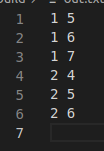
\includegraphics[width=0.25\textwidth]{img/res_word.png}
	\caption{Пример №1, поиск подстроки word}
	\label{fig:test-01}
\end{figure}

\begin{figure}[h]
	\centering
	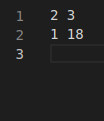
\includegraphics[width=0.25\textwidth]{img/res_m.png}
	\caption{Пример №2, поиск подстроки m}
	\label{fig:test-02}
\end{figure}
